\section*{Đề thi thử THPTQG Sở GD\&ĐT Quảng Ngai - Trường THPT Chuyên Lê Khiết - 25--26, Lần 1}
\caulc
\Opensolutionfile{ans}[ans/10-CK1-Chuyen-Hung-Vuong-Phan-1]
\begin{ex}%[1D6N4-3]
	Bất phương trình $\log x < 1$ có tập nghiệm là
	\choice
	{\True $(0;10)$}
	{$(-\infty;10)$}
	{$(1;+\infty)$}
	{$(0;1)$}
	\loigiai{
		Ta có $\log x < 1 \Leftrightarrow 0 < x < 10$.\\
		Bất phương trình có tập nghiệm là $(0;10)$.
	}
\end{ex}

\begin{ex}%[2H5N2-5]
	Trong không gian $Oxyz$, tìm tọa độ giao điểm $I$ của đường thẳng $\Delta \colon \heva{&x=2-t\\ &y=3+t\\ &z=2t}$ và mặt phẳng $(\alpha) \colon x-2y+z-4=0$
	\choice
	{$I(2;3;0)$}
	{\True $I(10;-5;-16)$}
	{$I(-7;5;2)$}
	{$I(1;-2;1)$}
	\loigiai{
		Xét phương trình $2-t-2(3+t)+2t-4=0 \Leftrightarrow t=-8$.\\
		Vậy tọa độ giao điểm $I(10;-5;-16)$.
	}
\end{ex}

\begin{ex}%[1D2N2-4]
	Cho cấp số cộng $(u_n)$ thỏa mãn $u_1+u_7=12$, số hạng $u_1$ của cấp số cộng đó bằng
	\choice
	{$8$}
	{\True $6$}
	{$12$}
	{$4$}
	\loigiai{
		Từ $u_1+u_7=12 \Leftrightarrow u_1+(u_1+6d)=12 \Leftrightarrow u_1+3d=6 \Leftrightarrow u_4=6$.
	}
\end{ex}

\begin{ex}%[2D1N5-1]
	Hàm số nào dưới đây có đồ thị là đường cong hình vẽ?
	\begin{center}
		\begin{tikzpicture}[scale=0.7,font=\footnotesize,line join=round,line cap=round,>=stealth]
			\draw[->] (-4.5,0) -- (4,0) node[below] {$x$};
			\draw[->] (0,-4) -- (0,3) node[right] {$y$};
			\path (0,0) node[below left] {$O$};
			
			\draw (-1,-4) -- (-1,3);
			\draw (-4.5,-2) -- (4,-2);
			
			\draw[fill=black] (0,1) circle(1pt) node[right] {$1$};
			\path (-1,0) node[above left] {$-1$};
			\path (0,-2) node[below right] {$-2$};
			
			\clip (-4.5,-4) rectangle (4,3);
			\draw[smooth,samples=200,domain=-4.5:-1.05] plot(\x,{(-2*\x+1)/(\x+1)});
			\draw[smooth,samples=200,domain=-0.95:4] plot(\x,{(-2*\x+1)/(\x+1)});
		\end{tikzpicture}
	\end{center}
	\choice
	{$y=\dfrac{-2x-1}{x+1}$}
	{$y=\dfrac{x-1}{x+1}$}
	{\True $y=\dfrac{-2x+1}{x+1}$}
	{$y=\dfrac{x+1}{x-1}$}
	\loigiai{
		Vì đồ thị có tiệm cận đứng $x=-1$, tiệm cận ngang $y=-2$, đi qua điểm $A(0;1)$ trên trục $Oy$ nên hàm số là $y=\dfrac{-2x+1}{x+1}$.
	}
\end{ex}

\begin{ex}%[2D4H2-2]
	Cho hàm số $f(x)=x^2-\dfrac{4}{x}$. Giá trị của $\displaystyle\int\limits_1^2 f'(x) \mathrm{\,d}x$ bằng
	\choice
	{$5-\ln 2$}
	{$\dfrac{7}{2}-\ln 2$}
	{\True $5$}
	{$\dfrac{7}{3}$}
	\loigiai{
		Ta có $\displaystyle\int\limits_1^2 f'(x)\mathrm{\,d}x = f(x)\big|_1^2 = f(2)-f(1) = 2^2-\dfrac{4}{2} - \left(1^2-\dfrac{4}{1}\right) = 5$.
	}
\end{ex}

\begin{ex}%[2D3H1-3]
	Theo thống kê điểm trung bình môn Toán của một số học sinh đã trúng tuyển vào lớp $10$ tại một trường học năm học $2025$ - $2026$, thu được kết quả như bảng sau:
	\begin{center}
		\begin{tabular}{|c|c|c|c|c|c|c|c|}
			\hline
			Khoảng điểm & $[6{,}5; 7)$ & $[7; 7{,}5)$ & $[7{,}5; 8)$ & $[8; 8{,}5)$ & $[8{,}5; 9)$ & $[9; 9{,}5)$ & $[9{,}5; 10)$ \\
			\hline
			Tần số & $7$ & $10$ & $17$ & $24$ & $13$ & $8$ & $5$ \\
			\hline
		\end{tabular}
	\end{center}
	Khoảng tứ phân vị của mẫu số liệu ghép nhóm trên gần nhất với kết quả nào sau đây?
	\choice
	{\True $\Delta_Q=1{,}1$}
	{$\Delta_Q=1{,}2$}
	{$\Delta_Q=1$}
	{$\Delta_Q=0{,}6$}
	\loigiai{
		Ta lập bảng tần số tích lũy của mẫu số liệu
		\begin{center}
			\begin{tabular}{|c|c|c|c|c|c|c|c|}
				\hline
				Khoảng điểm & $[6{,}5; 7)$ & $[7; 7{,}5)$ & $[7{,}5; 8)$ & $[8; 8{,}5)$ & $[8{,}5; 9)$ & $[9; 9{,}5)$ & $[9{,}5; 10)$ \\
				\hline
				Tần số & $7$ & $10$ & $17$ & $24$ & $13$ & $8$ & $5$ \\
				\hline
				Tần số tích lũy & $7$ & $17$ & $34$ & $58$ & $71$ & $79$ & $84$ \\
				\hline
			\end{tabular}
		\end{center}
		Cỡ mẫu là $N = 84$.\\
		Gọi $x_1$; $x_2$; $\ldots$; $x_{84}$ là điểm số của $84$ học sinh và giả sử dãy số liệu được sắp xếp theo thứ tự không giảm.\\
		Tứ phân vị thứ nhất $Q_1$ là trung vị của nửa số liệu bên trái $Q_2$, suy ra $Q_1 = \dfrac{x_{21} + x_{22}}{2}$.\\
		Giá trị $x_{21}$ và $x_{22}$ đều thuộc nhóm $[7{,}5; 8)$. Nhóm chứa $Q_1$ là $[7{,}5; 8)$.\\
		Ta có
		$$Q_1 = 7{,}5 + \dfrac{\dfrac{84}{4} - 17}{17} \cdot 0{,}5 = 7{,}5 + \dfrac{21 - 17}{17} \cdot 0{,}5 = \dfrac{259}{34}.$$
		Tứ phân vị thứ ba $Q_3$ là trung vị của nửa số liệu bên phải $Q_2$, suy ra $Q_3 = \dfrac{x_{63} + x_{64}}{2}$.\\
		Giá trị $x_{63}$ thuộc nhóm $[8{,}5; 9)$ và $x_{64}$ cũng thuộc nhóm $[8{,}5; 9)$. Nhóm chứa $Q_3$ là $[8{,}5; 9)$.\\
		Ta có
		$$Q_3 = 8{,}5 + \dfrac{\dfrac{3 \cdot 84}{4} - 58}{13} \cdot 0{,}5 = 8{,}5 + \dfrac{63 - 58}{13} \cdot 0{,}5 = \dfrac{113}{13}.$$
		Khoảng tứ phân vị của mẫu số liệu ghép nhóm là
		$$\Delta_Q = Q_3 - Q_1 = \dfrac{113}{13} - \dfrac{259}{34} = \dfrac{475}{442} \approx 1{,}0746 \approx 1{,}1.$$
	}
\end{ex}

\begin{ex}%[2D4H3-1]
	Diện tích hình phẳng tô đậm trong hình vẽ bên bằng
	\begin{center}
		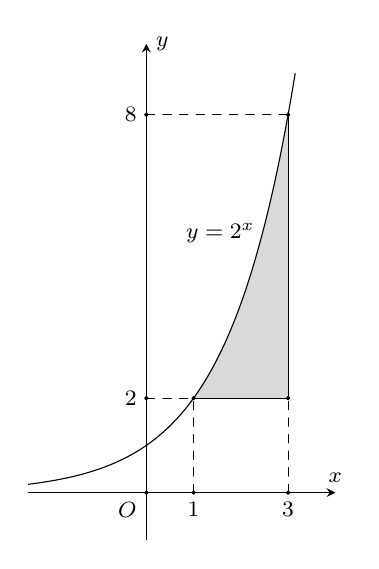
\begin{tikzpicture}[scale=0.6,font=\footnotesize,line join=round,line cap=round,>=stealth]
			\fill[gray!30] (1,2) -- plot[domain=1:3] (\x,{2^\x}) -- (3,8) -- (3,2) -- cycle;
			
			\draw[->] (-2.5,0) -- (4,0) node[above] {$x$};
			\draw[->] (0,-1) -- (0,9.5) node[right] {$y$};
			\path (0,0) node[below left] {$O$};
			
			\draw[smooth,samples=100,domain=-2.5:3.15] plot(\x,{2^\x});
			\path (2.5,5.5) node[left] {$y=2^x$};
			
			\draw[dashed] (0,8) node[left] {$8$} -- (3,8);
			\draw[dashed] (0,2) node[left] {$2$} -- (1,2);
			\draw (1,2) -- (3,2) -- (3,8);
			\draw[dashed] (1,0) node[below] {$1$} -- (1,2);
			\draw[dashed] (3,0) node[below] {$3$} -- (3,2);
			
			\foreach \p in {(0,0), (1,0), (3,0), (0,2), (0,8), (1,2), (3,2), (3,8)}
			\draw[fill=black] \p circle(1pt);
		\end{tikzpicture}
	\end{center}
	\choice
	{$\displaystyle\int\limits_1^3 2^x \mathrm{d}x$}
	{$\displaystyle\int\limits_1^3 \left(2^x+2\right) \mathrm{d}x$}
	{\True $\displaystyle\int\limits_1^3 \left(2^x-2\right) \mathrm{d}x$}
	{$\displaystyle\int\limits_1^3 \left(2-2^x\right) \mathrm{d}x$}
	\loigiai{
		Dựa vào hình vẽ, diện tích hình phẳng tô đậm được giới hạn bởi\\
		Đồ thị hàm số $y=2^x$ (là đường cong phía trên);\\
		Đường thẳng $y=2$ (là đường thẳng nằm ngang phía dưới);\\
		Hai đường thẳng đứng $x=1$ và $x=3$.\\
		Vậy diện tích hình phẳng tô đậm là $S = \displaystyle\int\limits_1^3 \left(2^x-2\right)\mathrm{d}x$.
	}
\end{ex}

\begin{ex}%[1H8H6-1]
	Cho hình lập phương $ABCD.A'B'C'D'$ (tham khảo hình bên). Giá trị $\sin$ của góc giữa đường thẳng $AC'$ và mặt phẳng $(ABCD)$ bằng
	\begin{center}
		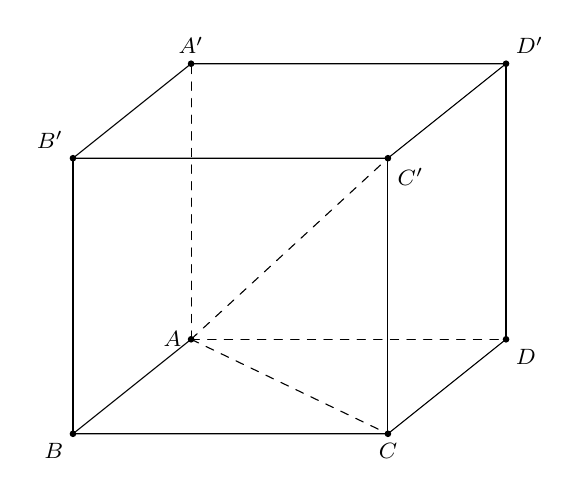
\begin{tikzpicture}[scale=1,font=\footnotesize,line join=round,line cap=round,>=stealth]
			\coordinate (A) at (0,0);
			\coordinate (B) at (-1.5,-1.2);
			\coordinate (C) at (2.5,-1.2);
			\coordinate (D) at (4,0);
			\coordinate (A') at (0,3.5);
			\coordinate (B') at (-1.5,2.3);
			\coordinate (C') at (2.5,2.3);
			\coordinate (D') at (4,3.5);
			
			\draw (A) -- (B) -- (C) -- (D);
			\draw (A') -- (B') -- (C') -- (D') -- cycle;
			\draw (B) -- (B');
			\draw (C) -- (C');
			\draw (D) -- (D');
			
			\draw[dashed] (A) -- (D);
			\draw[dashed] (A) -- (A');
			\draw[dashed] (A) -- (C);
			\draw[dashed] (A) -- (C');
			
			\foreach \p in {A,B,C,D,A',B',C',D'}
			\fill (\p) circle (1.2pt);
			
			\path (A) node[left] {$A$};
			\path (B) node[below left] {$B$};
			\path (C) node[below] {$C$};
			\path (D) node[below right] {$D$};
			\path (A') node[above] {$A'$};
			\path (B') node[above left] {$B'$};
			\path (C') node[below right] {$C'$};
			\path (D') node[above right] {$D'$};
		\end{tikzpicture}
	\end{center}
	\choice
	{$\dfrac{\sqrt{3}}{2}$}
	{$\dfrac{\sqrt{6}}{3}$}
	{\True $\dfrac{\sqrt{3}}{3}$}
	{$\dfrac{\sqrt{2}}{2}$}
	\loigiai{
		Hình chiếu của đường thẳng $AC'$ lên mặt phẳng $(ABCD)$ là đường thẳng $AC$.\\
		Góc giữa đường thẳng $AC'$ và mặt phẳng $(ABCD)$ chính là góc giữa đường thẳng $AC'$ và hình chiếu $AC$ của nó.\\
		Ký hiệu góc đó là $\alpha = \widehat{C'AC}$.\\
		Tam giác $C'CA$ vuông tại $C$. Gọi độ dài cạnh của hình lập phương là $a$.\\
		Khi đó $CC' = a$.\\
		$AC$ là đường chéo của hình vuông $ABCD$ có cạnh $a$.\\
		Do đó $AC = \sqrt{a^2+a^2} = \sqrt{2a^2} = a\sqrt{2}$.\\
		$AC' = \sqrt{a^2+(a\sqrt{2})^2} = a\sqrt{3}$.\\
		Trong tam giác vuông $C'CA$, ta có $\sin \widehat{C'AC} = \dfrac{a}{a\sqrt{3}} = \dfrac{\sqrt{3}}{3}$.\\
		Vậy giá trị $\sin$ của góc giữa đường thẳng $AC'$ và mặt phẳng $(ABCD)$ là $\dfrac{\sqrt{3}}{3}$.
	}
\end{ex}

\begin{ex}%[1H8H1-3]
	Cho hình chóp $S.ABC$ có đáy là tam giác $ABC$ đều, $SA=AB=a$. Gọi $E$, $F$ lần lượt là trung điểm của $SB$, $SC$. Khi đó góc giữa $EF$ và $AB$ bằng
	\choice
	{\True $60^\circ$}
	{$45^\circ$}
	{$30^\circ$}
	{$90^\circ$}
	\loigiai{
		\begin{center}
			\begin{tikzpicture}[line join=round, line cap=round, scale=1]
				\coordinate (A) at (0,0);
				\coordinate (C) at (6,0);
				\coordinate (B) at (1.5,-2);
				\coordinate (S) at (0.8,4.5);
				
				\path (S) -- (B) coordinate[pos=0.5] (E);
				\path (S) -- (C) coordinate[pos=0.5] (F);
				
				\draw[dashed] (A) -- (C);
				
				\draw (S) -- (A);
				\draw (S) -- (B);
				\draw (S) -- (C);
				\draw (A) -- (B);
				\draw (B) -- (C);
				\draw (E) -- (F);
				
				\node[left] at (A) {$A$};
				\node[below left] at (B) {$B$};
				\node[below right] at (C) {$C$};
				\node[above] at (S) {$S$};
				\node[left=0.1cm] at (E) {$E$};
				\node[above right=0.05cm] at (F) {$F$};
			\end{tikzpicture}
		\end{center}
		Xét $\triangle SBC$, ta có $E$ và $F$ lần lượt là trung điểm của $SB$ và $SC$. \\
		Suy ra $EF$ là đường trung bình của $\triangle SBC$. \\
		Do đó, $EF \parallel BC$.\\
		Vì $EF \parallel BC$ nên góc giữa hai đường thẳng $EF$ và $AB$ bằng góc giữa hai đường thẳng $BC$ và $AB$ hay $(EF, AB) = (BC, AB)$.\\
		Theo giả thiết, $\triangle ABC$ là tam giác đều nên $\widehat{ABC} = 60^\circ$.\\
		Vì $0^\circ < \widehat{ABC} \le 90^\circ$ nên góc giữa hai đường thẳng $AB$ và $BC$ chính là số đo của góc $\widehat{ABC}$. \\
		Vậy $(EF, AB) = (BC, AB) = \widehat{ABC} = 60^\circ$.
	}
\end{ex}

\begin{ex}%[1D6N3-1]
	Cho $f(x)=5^x$ thì $f(x+1)-f(x)$ bằng
	\choice
	{$4$}
	{\True $4f(x)$}
	{$5f(x)$}
	{$5$}
	\loigiai{
		Ta có $f(x+1)-f(x) = 5^{x+1}-5^x = 4 \cdot 5^x = 4f(x)$.
	}
\end{ex}

\begin{ex}%[2H5N1-3]
	Trong không gian $Oxyz$, cho điểm $H(m;n;1)$ thuộc mặt phẳng $(\alpha) \colon x+2y-z+3=0$. Mệnh đề nào đúng?
	\choice
	{$m+2n=4$}
	{\True $m+2n=-2$}
	{$m+2n=2$}
	{$m+2n=-4$}
	\loigiai{
		Điểm $H(m;n;1)$ thuộc mặt phẳng $(\alpha) \colon x+2y-z+3=0 \Rightarrow m+2n-1+3=0 \Leftrightarrow m+2n=-2$.
	}
\end{ex}

\begin{ex}%[2D1N1-2]
	Cho hàm số $y=f(x)$ có bảng biến thiên như hình vẽ. Hàm số $y=f(x)$ nghịch biến trên khoảng nào dưới đây?
	\begin{center}
		
\begin{tikzpicture}
			\tkzTabInit[nocadre=false,lgt=1.2,espcl=2]{$x$/0.6, $y'$/0.6, $y$/2}{$-\infty$, $-2$, $0$, $2$, $+\infty$}
			\tkzTabLine{ , +, 0, -, 0, +, 0, -, }
			\tkzTabVar{-/ $-\infty$, +/ $3$, -/ $-1$, +/ $3$, -/ $-\infty$}
		\end{tikzpicture}
	\end{center}
	\choice
	{\True $(2;4)$}
	{$(0;2)$}
	{$(0;+\infty)$}
	{$(-\infty;2)$}
	\loigiai{
		Từ bảng biến thiên suy ra hàm số $y=f(x)$ nghịch biến trên $(2;+\infty)$, suy ra hàm số nghịch biến trên $(2;4)$.
	}
\end{ex}

\Closesolutionfile{ans}

\cauds
\Opensolutionfile{ans}[ans/10-CK1-Chuyen-Hung-Vuong-Phan-2]
\begin{ex}%[2D1H2-7]
	Một đại lý xăng dầu tại Quảng Ngãi cần làm một bồn chứa dầu hình trụ bằng tôn có thể tích $V=54\pi$ (m$^3$). Gọi $r$, $h$ lần lượt là bán kính đáy và chiều cao của cái bồn dầu.
	\choiceTF
	{\True Công thức để tính thể tích bồn chứa dầu là $V=\pi r^2 h$}
	{\True Để diện tích toàn phần nhỏ nhất thì bán kính $r=3$ (m)}
	{\True Diện tích toàn phần của bồn chứa dầu theo bán kính $r$ là $S(r)=2\pi\left(\dfrac{54}{r}+r^2\right)$}
	{Biết chi phí vật liệu (tôn) để làm bồn chứa là $500\,000$ đồng/m$^2$. Khi đó, số tiền ít nhất để mua nguyên vật liệu làm bồn chứa dầu là khoảng $81$ triệu đồng (làm tròn đến hàng phần mười)}
	\loigiai{
		\begin{itemchoice}
			\itemch Công thức để tính thể tích bồn chứa dầu là $V=\pi r^2 h$.
			\itemch Ta có $V = \pi r^2 h = 54\pi \Leftrightarrow h = \dfrac{54}{r^2}$.\\
			Diện tích xung quanh của hình trụ là $S_{xq} = 2\pi rh = 2\pi r \cdot \dfrac{54}{r^2} = \dfrac{108\pi}{r}$.\\
			Diện tích toàn phần của hình trụ là $S_{tp} = 2\pi rh + 2\pi r^2 = \dfrac{108\pi}{r} + 2\pi r^2 = 2\pi\left(\dfrac{54}{r} + r^2\right)$.\\
			Xét hàm số $f(x) = x^2 + \dfrac{54}{x}$ với $x > 0$.\\
			$f'(x) = 2x - \dfrac{54}{x^2} = 0 \Leftrightarrow x = 3$.
			\begin{center}
				\begin{center}
					
\begin{tikzpicture}
						\tkzTabInit[nocadre=false,lgt=1.2,espcl=2.5,deltacl=0.6]{$x$/0.8, $f'(x)$/0.8, $f(x)$/2}{$0$, $3$, $+\infty$}
						\tkzTabLine{ , -, 0, +, }
						\tkzTabVar{+/ , -/ $f(3)$, +/ }
					\end{tikzpicture}
				\end{center}
			\end{center}
			Hàm số $y = f(x)$ đạt GTNN trên $(0;+\infty)$ khi $x=3$.\\
			Vậy để diện tích toàn phần nhỏ nhất thì bán kính $r=3$ (m).
			\itemch Diện tích toàn phần của hình trụ là $S_{tp} = 2\pi\left(\dfrac{54}{r} + r^2\right)$.
			\itemch Diện tích toàn phần của bồn nước nhỏ nhất là $S(3) = 2\pi\left(\dfrac{54}{3} + 3^2\right) = 54\pi$ (m$^2$).\\
			Số tiền mua nguyên vật liệu ít nhất là $54\pi \cdot 500\,000 \approx 84\,823\,001$ (đồng) $\approx 85$ (triệu đồng).
		\end{itemchoice}
	}
\end{ex}

\begin{ex}%[2H5H3-4]
	Xét một hệ trục tọa độ $Oxyz$ được cho sẵn, đơn vị trên mỗi trục là dm, mặt ngoài của một cục đá có dạng hình cầu được mô hình hóa bởi phương trình mặt cầu\break $(x-2)^2+(y+1)^2+(z+1)^2=6$, cục đá nằm yên trên sàn nhà. Người ta nhìn thấy một tấm ván ngã xuống đè lên cục đá, phần giao của tấm ván và sàn nhà là đường thẳng $d$ có phương trình $\dfrac{x+2}{2}=\dfrac{y+1}{-3}=\dfrac{z}{1}$. Gọi $A$, $B$ lần lượt là hai tiếp điểm của tấm ván, sàn nhà với cục đá và $I$ là tâm cục đá (hình vẽ minh họa).
	\begin{center}
		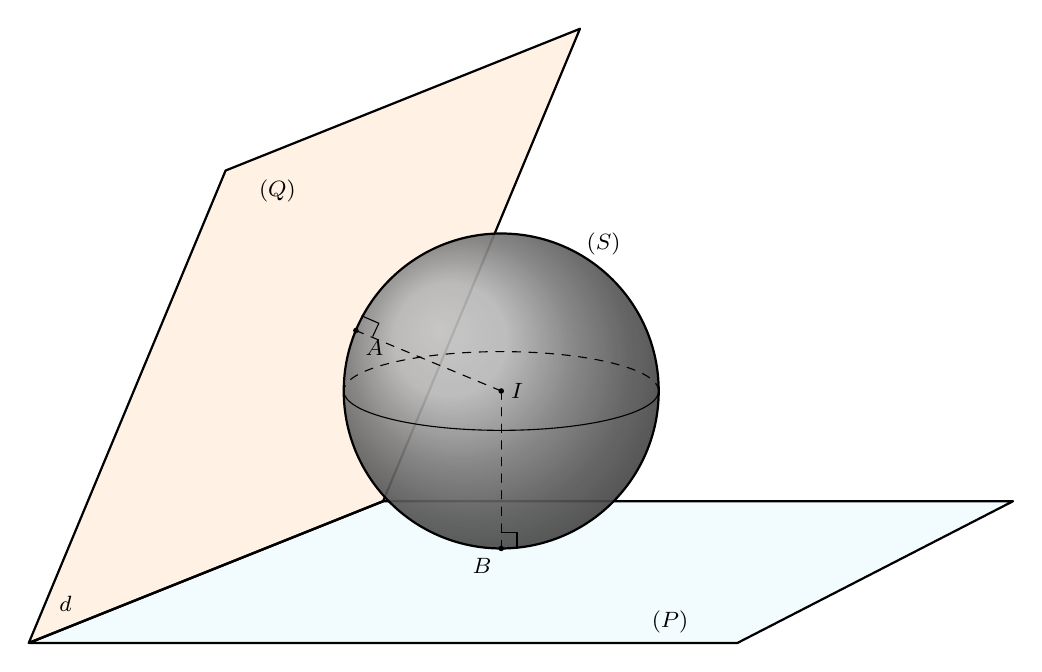
\begin{tikzpicture}[scale=1,font=\footnotesize,line join=round,line cap=round,>=stealth]
			\coordinate (I) at (1.5, 2.6);
			\coordinate (B) at (1.5, 0.6);
			\coordinate (A) at (-0.346, 3.368);
			
			\coordinate (P1) at (-4.5, -0.6);
			\coordinate (P2) at (4.5, -0.6);
			\coordinate (P3) at (8, 1.2);
			\coordinate (P4) at (0, 1.2);
			
			\coordinate (Q1) at (-4.5, -0.6);
			\coordinate (Q2) at (-2.0, 5.4);
			\coordinate (Q3) at (2.5, 7.2);
			\coordinate (Q4) at (0, 1.2);
			
			\fill[cyan!5] (P1) -- (P2) -- (P3) -- (P4) -- cycle;
			\draw[thick] (P1) -- (P2) -- (P3) -- (P4) -- cycle;
			\path (P2) node[above left, xshift=-0.5cm] {$(P)$};
			
			\fill[orange!20, opacity=0.5] (Q1) -- (Q2) -- (Q3) -- (Q4) -- cycle;
			\draw[thick] (Q1) -- (Q2) -- (Q3) -- (Q4) -- cycle;
			\path (Q2) node[below right, xshift=0.3cm] {$(Q)$};
			
			\draw[thick] (P1) -- (P4) node[pos=0.15, above left] {$d$};
			
			\fill[ball color=gray!20, opacity=0.7] (I) circle (2);
			\draw[thick] (I) circle (2);
			\node[above] at (2.8, 4.2) {$(S)$};
			
			\draw[dashed] (I) -- (A);
			\draw[dashed] (I) -- (B);
			
			\draw (1.5, 0.8) -- (1.7, 0.8) -- (1.7, 0.6);
			\draw (-0.269, 3.553) -- (-0.454+0.4, 3.630-0.17) -- (-0.531+0.4, 3.445-0.15);
			
			\draw[dashed] (3.5, 2.6) arc (0:180:2 and 0.5);
			\draw (-0.5, 2.6) arc (180:360:2 and 0.5);
			
			\fill (I) circle (1pt) node[right] {$I$};
			\fill (B) circle (1pt) node[below left] {$B$};
			\fill (A) circle (1pt) node[below right] {$A$};
		\end{tikzpicture}
	\end{center}
	\choiceTF
	{\True Tâm $I(2;-1;-1)$ và bán kính $R=\sqrt{6}$}
	{Khoảng cách từ tâm $I$ đến đường thẳng $d$ bằng $2\sqrt{6}$}
	{\True Nếu $\cos \widehat{AIB}$ bằng $\dfrac{a}{b}$ (phân số tối giản) thì giá trị $a^2+b^2=82$}
	{\True Giả sử tại các điểm $A$ và $B$ trên cục đá có các khe hở nhỏ vừa đủ cho một con kiến lách qua. Một con kiến bò trên bề mặt ngoài của cục đá từ $A$ đến $B$ với tốc độ không đổi $2$ cm/s, thời gian ngắn nhất cho chuyến đi này là $21$ giây (làm tròn đến hàng đơn vị)}
	\loigiai{
		\begin{itemchoice}
			\itemch Tâm $I(2;-1;-1)$ và bán kính $R=\sqrt{6}$.
			\itemch Phương trình tham số của đường thẳng $d$ là $\heva{&x = -2 + 2t \\ &y = -1 - 3t \\ &z = t.}$\\
			Gọi $H$ là hình chiếu vuông góc của $I$ lên đường thẳng $d$.\\
			Vì $H \in d$ nên $H(-2 + 2t; -1 - 3t; t)$.\\
			Suy ra $\overrightarrow{IH} = (-4 + 2t; -3t; t + 1)$.\\
			Đường thẳng $d$ có một vectơ chỉ phương là $\overrightarrow{u}=(2;-3;1)$.\\
			Vì $IH \perp d$ nên $\overrightarrow{IH} \cdot \overrightarrow{u} = 0$\\
			$\Leftrightarrow 2(-4 + 2t) - 3(-3t) + 1(t + 1) = 0$\\
			$\Leftrightarrow -8 + 4t + 9t + t + 1 = 0$\\
			$\Leftrightarrow 14t - 7 = 0 \Leftrightarrow t = \dfrac{1}{2}$.\\
			Khi đó $\overrightarrow{IH} = \left(-3; -\dfrac{3}{2}; \dfrac{3}{2}\right)$.\\
			Khoảng cách từ tâm $I$ đến đường thẳng $d$ là:\\
			$$\mathrm{d}(I,d) = IH = \left|\overrightarrow{IH}\right| = \sqrt{(-3)^2+\left(-\dfrac{3}{2}\right)^2+\left(\dfrac{3}{2}\right)^2} = \dfrac{3\sqrt{6}}{2}.$$
			\itemch Đường thẳng $d$ là giao tuyến của mặt sàn và tấm ván.\\
			Gọi $H$ là hình chiếu vuông góc của $I$ lên $d$.\\
			Mà $A$, $B$ là các tiếp điểm của tấm ván và mặt sàn với mặt cầu, suy ra $HA \perp IA$, $HB \perp IB$.\\
			Do đó, $HA$, $HB$ là hai tiếp tuyến cắt nhau.\\
			Suy ra $\widehat{AIH} = \widehat{BIH}$ hay $\widehat{AIB} = 2\widehat{AIH}$.\\
			Ta có $IH = \mathrm{d}(I,d) = \dfrac{3\sqrt{6}}{2}$.\\
			Xét tam giác $AIH$ vuông tại $A$, ta có $\cos \widehat{AIH} = \dfrac{IA}{IH} = \dfrac{\sqrt{6}}{\dfrac{3\sqrt{6}}{2}} = \dfrac{2}{3}$.\\
			Suy ra $\cos \widehat{AIB} = \cos \left(2\widehat{AIH}\right) = 2\cos^2\widehat{AIH} - 1 = 2 \cdot \left(\dfrac{2}{3}\right)^2 - 1 = -\dfrac{1}{9}$.\\
			Vậy $a=-1$, $b=9 \Rightarrow a^2+b^2 = (-1)^2+9^2 = 82$.
			\itemch Để thời gian con kiến bò là ngắn nhất, quãng đường đi từ $A$ đến $B$ trên bề mặt cục đá phải là cung nhỏ $AB$ của đường tròn lớn đi qua $A$ và $B$.\\
			Bán kính đường tròn lớn là bán kính mặt cầu
			$$R=\sqrt{6} \text{ dm} = 10\sqrt{6} \text{ cm}.$$
			Góc ở tâm chắn cung nhỏ $AB$ là $\alpha = \arccos\left(-\dfrac{1}{9}\right) \approx 1{,}682$ (rad).\\
			Độ dài quãng đường ngắn nhất là độ dài cung $AB$ là $S = R \cdot \alpha = 10\sqrt{6} \cdot 1{,}682 \approx 41{,}204$ (cm).\\
			Thời gian ngắn nhất để con kiến hoàn thành chuyến đi là $t = \dfrac{S}{v} = \dfrac{41{,}204}{2} \approx 21$ (giây).
		\end{itemchoice}
	}
\end{ex}

\begin{ex}%[2D4H1-6]
	Một cốc cà phê nóng có nhiệt độ ban đầu là $80^\circ$C được đặt trong một phòng có nhiệt độ ổn định $20^\circ$C. Sau $15$ phút, nhiệt độ của cốc cà phê giảm xuống còn $50^\circ$C. Gọi $T(t)$ là nhiệt độ của cốc cà phê tại thời điểm $t$ (phút) và $y(t)=T(t)-20$ là chênh lệch nhiệt độ giữa cà phê và môi trường. Biết rằng tốc độ thay đổi chênh lệch nhiệt độ tỉ lệ thuận với chính nó, tức là $y'(t)=k\cdot y(t)$ (với $k$ là hằng số).
	\choiceTF
	{\True Hằng số tốc độ làm mát của cốc cà phê $k=\dfrac{1}{15}\ln 2$}
	{Sau $30$ phút kể từ khi đặt vào phòng, nhiệt độ của cốc cà phê là $30^\circ$C (làm tròn đến hàng đơn vị)}
	{\True $y(t)=60e^{kt}$ với mọi $t \ge 0$}
	{\True Tại thời điểm ban đầu ($t=0$), giá trị của hằng số $C$ trong biểu thức $y(t)=e^{kt+C}$ là $C=\ln 60$}
	\loigiai{
		\begin{itemchoice}
			\itemch Ta có $y'(t)=k \cdot y(t) \Rightarrow \displaystyle\int \dfrac{y'(t)}{y(t)} \,\mathrm{\,d}t = \displaystyle\int k \,\mathrm{\,d}t \Rightarrow \ln|y(t)| = kt+C$.\\
			Do đó $y(t) = e^{kt+C}$.\\
			Mà $y(t) = T(t)-20$ nên $T(t) = e^{kt+C}+20$.\\
			Ta có $\heva{&T(15) = e^{k \cdot 15+C}+20=50\\ &T(0) = e^{k \cdot 0+C}+20=80} \Leftrightarrow \heva{&e^{k \cdot 15+C}=30\\ &e^C=60} \Leftrightarrow \heva{&k \cdot 15+C=\ln 30\\ &C=\ln 60} \Leftrightarrow \heva{&k=-\dfrac{1}{15}\ln 2\\ &C=\ln 60.}$\\
			Hằng số tốc độ làm mát của cốc cà phê $k=\dfrac{1}{15}\ln 2$.
			\itemch Sau $30$ phút, nhiệt độ của cốc cà phê là $T(30) = e^{-\tfrac{1}{15}\ln 2 \cdot 30 + \ln 60} + 20 = 35$ ($^\circ$C).
			\itemch Với $C=\ln 60 \Rightarrow y(t) = e^{kt+\ln 60} = 60 \cdot e^{kt}$.
			\itemch Tại thời điểm ban đầu ($t=0$), giá trị của hằng số $C$ trong biểu thức $y(t)=e^{kt+C}$ là $C=\ln 60$.
		\end{itemchoice}
	}
\end{ex}

\begin{ex}%[2D6H2-4]
	Hộp $X$ có $5$ bi đen và $5$ bi trắng, hộp $Y$ có $6$ bi đen và $8$ bi trắng. Bạn $H$ lấy ngẫu nhiên $2$ viên bi từ hộp $X$ bỏ sang hộp $Y$, sau đó tiếp tục lấy ngẫu nhiên $3$ viên bi từ hộp $Y$ (hình vẽ minh họa).
	\choiceTF
	{\True Biết rằng bạn $H$ đã lấy được $2$ viên bi đen và $1$ viên bi trắng từ hộp $Y$, xác suất để $2$ viên bi đen ấy là từ hộp $X$ chuyển qua bằng $\dfrac{448}{1693}$}
	{\True Xác suất để lấy được $3$ viên bi đen từ hộp $Y$ bằng $\dfrac{109}{1680}$}
	{\True Xác suất lấy được $2$ viên bi đen và $1$ viên bi trắng từ hộp $Y$ bằng $\dfrac{1693}{5040}$}
	{Xác suất để lấy được $2$ viên bi trắng từ hộp $X$ bằng $\dfrac{1}{3}$}
	\loigiai{
		\begin{itemchoice}
			\itemch Trong hộp $X$ có $10$ viên bi trong đó có $5$ viên bi trắng và $5$ bi đen nên xác suất lấy $2$ viên bi trắng từ hộp $X$ là $P = \dfrac{\mathrm{C}_5^2}{\mathrm{C}_{10}^2} = \dfrac{2}{9}$.
			\itemch Lấy hai viên bi từ hộp $X$ cho sang hộp $Y$ có $3$ trường hợp xảy ra.
			\begin{enumerate}[TH 1.]
				\item Lấy $2$ viên bi đen từ hộp $X$ sang hộp $Y$\\
				Ta có $\mathrm{P}=\dfrac{\mathrm{C}_5^2}{\mathrm{C}_{10}^2}=\dfrac{2}{9}$.\\
				Khi đó hộp $Y$ có $8$ bi đen, $8$ bi trắng, khi đó xác suất lấy $3$ bi đen từ hộp $Y$ là $\dfrac{\mathrm{C}_8^3}{\mathrm{C}_{16}^3} = \dfrac{1}{10}$.
				\item Lấy $1$ bi trắng và $1$ bi đen từ hộp $X$ cho sang hộp $Y$\\
				Ta có $\mathrm{P}=\dfrac{5 \cdot 5}{\mathrm{C}_{10}^2}=\dfrac{5}{9}$.\\
				Khi đó hộp $Y$ có $7$ bi đen, $9$ bi trắng, khi đó xác suất lấy $3$ bi đen từ hộp $Y$ là $\dfrac{\mathrm{C}_7^3}{\mathrm{C}_{16}^3} = \dfrac{1}{16}$.
				\item Lấy $2$ bi trắng từ hộp $X$ sang hộp $Y$\\
				Ta có $\mathrm{P}=\dfrac{\mathrm{C}_5^2}{\mathrm{C}_{10}^2}=\dfrac{2}{9}$.\\
				Khi đó hộp $Y$ có $6$ bi đen và $10$ bi trắng, khi đó xác suất lấy $3$ bi đen từ hộp $Y$ là $\dfrac{\mathrm{C}_6^3}{\mathrm{C}_{16}^3} = \dfrac{1}{28}$.
			\end{enumerate}
			Vậy xác suất để lấy $3$ viên bi đen từ hộp $Y$ là
			$$\mathrm{P} = \dfrac{2}{9} \cdot \dfrac{1}{10} + \dfrac{5}{9} \cdot \dfrac{1}{16} + \dfrac{2}{9} \cdot \dfrac{1}{28} = \dfrac{109}{1680}.$$
			\itemch Tương tự xác suất lấy $2$ bi đen và $1$ bi trắng ở hộp $Y$ là
			$$\mathrm{P} = \dfrac{2}{9} \cdot \dfrac{\mathrm{C}_8^2 \cdot 8}{\mathrm{C}_{16}^3} + \dfrac{5}{9} \cdot \dfrac{\mathrm{C}_7^2 \cdot 9}{\mathrm{C}_{16}^3} + \dfrac{2}{9} \cdot \dfrac{\mathrm{C}_6^2 \cdot 10}{\mathrm{C}_{16}^3} = \dfrac{1693}{5040}.$$
			\itemch Gọi $A$ là biến cố $H$ lấy được $2$ bi đen và $1$ bi trắng từ hộp $Y$.\\
			$B$ là biến cố lấy $2$ viên bi đen từ hộp $X$ chuyển sang.\\
			Khi đó biến cố \lq\lq Biết rằng bạn $H$ đã lấy được $2$ viên bi đen và $1$ viên bi trắng từ hộp $Y$\rq\rq, xác suất để 2 viên bi đen ấy là từ hộp $X$ chuyển qua là
			$$\mathrm{P} \left(B \mid A\right) = \dfrac{\mathrm{P}(A \cap B)}{P(A)} = \dfrac{\dfrac{448}{5040}}{\dfrac{1693}{5040}} = \dfrac{448}{1693}.$$
		\end{itemchoice}
	}
\end{ex}
\Closesolutionfile{ans}

\caukq
\Opensolutionfile{ans}[ans/10-CK1-Chuyen-Hung-Vuong-Phan-3]
\begin{ex}%[2D1H2-7]
	Một nhà máy chế tạo linh kiện điện tử đặc chủng, số lượng linh kiện được sản xuất mỗi tháng là $x$ ($x \in \mathbb{N}^*$, $100 \le x \le 5\,000$). Toàn bộ sản phẩm sản xuất ra đều được tiêu thụ với giá bán cố định là $200$ triệu đồng/linh kiện. Doanh thu được xác định theo mô hình tuyến tính $F(x)=200x$, tổng chi phí sản xuất lại tăng theo hàm mũ và được cho bởi công thức: $C(x)=100e^{0{,}001x}$ (đơn vị: triệu đồng). Để nhà máy đạt lợi nhuận tối thiểu là $25$ tỷ đồng, nhà máy cần sản xuất ít nhất bao nhiêu linh kiện trong tháng đó?
	\shortans{126}
	\loigiai{
		Lợi nhuận thu được của nhà máy trong tháng là
		$$L(x) = F(x) - C(x) = 200x - 100e^{0,001x} \text{ (triệu đồng)}.$$ 
		Để lợi nhuận tối thiểu là $25$ tỷ $= 25\,000$ triệu thì 
		$$L(x) \ge 25\,000 \Leftrightarrow 200x - 100e^{0{,}001x} - 25000 \ge 0.$$
		Xét hàm số $f(x) = 200x - 100e^{0{,}001x} - 25\,000$.\\
		Ta có $f'(x) = 200 - 0{,}1e^{0{,}001x}$.\\
		Với $100 \le x \le 5\,000$ thì $f'(x) \ge 200 - 0{,}1e^{5} > 0 \Rightarrow f(x)$ đồng biến.\\
		Ta có $f(125) \approx -113$ và $f(126) \approx 86{,}6$.\\
		Vì $x \in \mathbb{N}^*$ nên để $f(x) \ge 0$ thì $x \ge 126$.\\
		Vậy để nhà máy đạt lợi nhuận tối thiểu là $25$ tỷ đồng, nhà máy cần sản xuất ít nhất $126$ linh kiện trong tháng đó.
	}
\end{ex}

\begin{ex}%[0D2H2-3]
	Trong ngày hội trại $26/03$ vừa qua, chi đoàn lớp $12/1$ trường THPT $A$ tổ chức một gian hàng ẩm thực phục vụ thực khách với hai món chính là Trà đào và Nem chua rán. Để tăng doanh số, lớp thiết kế hai gói combo sau
	\begin{itemize}
		\item Combo \lq\lq Năng lượng\rq\rq: Giá $30$ nghìn đồng, bao gồm $1$ cốc trà đào và $1$ đĩa nem chua rán.
		\item Combo \lq\lq Bùng nổ\rq\rq: Giá $80$ nghìn đồng, bao gồm $2$ cốc trà đào và $3$ đĩa nem chua rán.
	\end{itemize}
	Qua tính toán nguyên liệu chuẩn bị ban đầu, lớp chỉ có thể phục vụ tối đa $120$ cốc trà đào và $150$ đĩa nem chua rán. Giả sử sức mua của học sinh và thầy cô trong trường là rất lớn, lớp luôn bán hết các combo đã đóng gói. Số tiền lớn nhất (đơn vị: nghìn đồng) mà chi đoàn lớp $12/1$ có thể thu được từ việc bán hai loại combo trên là bao nhiêu?
	\shortans{4200}
	\loigiai{
		Gọi số combo \lq\lq Năng lượng\rq\rq\ và combo \lq\lq Bùng nổ\rq\rq\ lần lượt là $x$, $y$ ($x$, $y \in \mathbb{N}$).\\
		Số cốc trà đào là $x+2y \le 120$.\\
		Số đĩa nem chua rán là $x+3y \le 150$.\\
		Số tiền thu được là $T(x;y) = 30x+80y$ (nghìn đồng).\\
		Ta có hệ điều kiện $\heva{&x,y \in \mathbb{N}\\ &x+2y \le 120\\ &x+3y \le 150.}$
		\begin{center}
			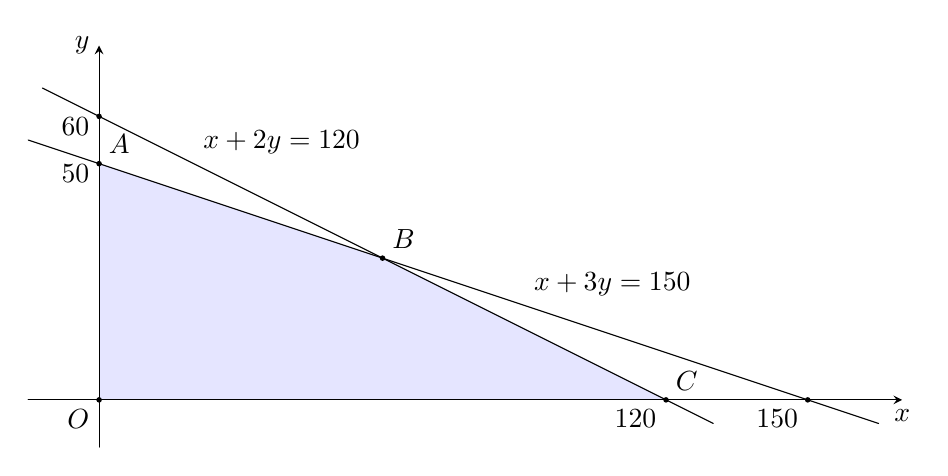
\begin{tikzpicture}[x=0.06cm,y=0.06cm,font=\normalsize,line join=round,line cap=round,>=stealth]
				\fill[blue!10] (0,0) -- (0,50) -- (60,30) -- (120,0) -- cycle;
				
				\draw (-12,66) -- (130,-5);
				\draw (-15,55) -- (165,-5);
				
				\draw[->] (-15,0) -- (170,0) node[below] {$x$};
				\draw[->] (0,-10) -- (0,75) node[left] {$y$};
				
				\path (20,50) node[above right] {$x + 2y = 120$};
				\path (90,20) node[above right] {$x + 3y = 150$};
				
				\fill (0,0) circle (1pt) node[below left] {$O$};
				\fill (0,50) circle (1pt) node[below left, yshift=3pt] {$50$} node[above right] {$A$};
				\fill (60,30) circle (1pt) node[above right] {$B$};
				\fill (120,0) circle (1pt) node[below left] {$120$} node[above right] {$C$};
				\fill (0,60) circle (1pt) node[below left, yshift=3pt] {$60$};
				\fill (150,0) circle (1pt) node[below left] {$150$};
			\end{tikzpicture}
		\end{center}
		Miền nghiệm của hệ là miền tứ giác $OABC$, với $O(0;0)$, $A(0;50)$, $C(120;0)$.\\
		Toạ độ điểm $B$ là $\heva{&x+2y=120\\ &x+3y=150} \Leftrightarrow \heva{&x=60\\ &y=30} \Rightarrow B(60;30)$.\\
		Ta có $T(O)=0$.\\
		$T(A) = 30 \cdot 50 + 80 \cdot 0 = 1\,500$.\\
		$T(B) = 30 \cdot 60 + 80 \cdot 30 = 4\,200$.\\
		$T(C) = 30 \cdot 120 = 3\,600$.\\
		Do đó, số tiền lớn nhất thu được là $4\,200$ nghìn đồng.
	}
\end{ex}

\begin{ex}%[1H8V7-4]
	Một công ty kiến trúc thiết kế một trạm dừng chân hiện đại có hình dáng là một khối lăng trụ tam giác $ABC.A'B'C'$, đảm bảo các yêu cầu sau
	\begin{itemize}
		\item Mặt sàn $(ABC)$ là một tam giác đều có cạnh bằng $6$ m.
		\item Cột trụ chính $AA'$ được đặt nghiêng sao cho hình chiếu vuông góc của đỉnh mái $A'$ lên mặt sàn $(ABC)$ trùng khớp với trọng tâm $G$ của tam giác $ABC$.
		\item Khoảng cách giữa cột trụ $AA'$ và mép sàn $BC$ là $1{,}5\sqrt{3}$ m.
	\end{itemize}
	Phần không gian giới hạn trong khối lăng trụ $ABC.A'B'C'$ có thể tích là $18\sqrt{m}$ (m$^3$). Giá trị của $m$ bằng bao nhiêu?
	\shortans{3}
	\loigiai{
		\begin{center}
			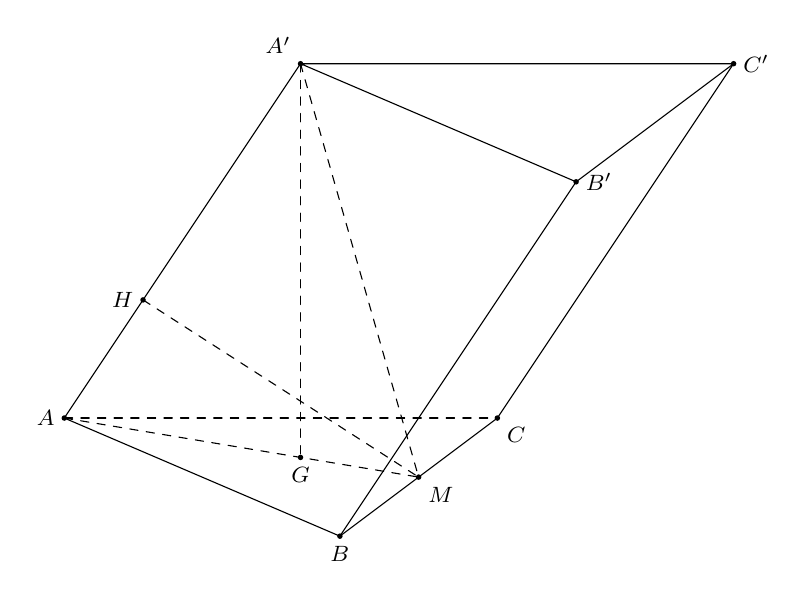
\begin{tikzpicture}[scale=1,font=\footnotesize,line join=round,line cap=round,>=stealth]
				\coordinate (A) at (0,0);
				\coordinate (B) at (3.5,-1.5);
				\coordinate (C) at (5.5,0);
				\coordinate (M) at (4.5,-0.75); 
				\coordinate (G) at (3,-0.5);    
				\coordinate (A') at (3,4.5);    
				\coordinate (B') at (6.5,3);    
				\coordinate (C') at (8.5,4.5);  
				\coordinate (H) at (1,1.5);     
				
				\draw (A) -- (B) -- (C);
				\draw (A') -- (B') -- (C') -- cycle;
				\draw (A) -- (A');
				\draw (B) -- (B');
				\draw (C) -- (C');
				
				\draw[dashed] (A) -- (C);
				\draw[dashed] (A) -- (M);
				\draw[dashed] (A') -- (G);
				\draw[dashed] (A') -- (M);
				\draw[dashed] (H) -- (M);
				
				\foreach \p in {A,B,C,A',B',C',M,G,H}
				\fill (\p) circle (1pt);
				
				\path (A) node[left] {$A$};
				\path (B) node[below] {$B$};
				\path (C) node[below right] {$C$};
				\path (A') node[above left] {$A'$};
				\path (B') node[right] {$B'$};
				\path (C') node[right] {$C'$};
				\path (M) node[below right] {$M$};
				\path (G) node[below] {$G$};
				\path (H) node[left] {$H$};
			\end{tikzpicture}
		\end{center}
		Mặt sàn $(ABC)$ là tam giác đều cạnh $a=6$ m.\\
		Diện tích đáy $S_{ABC} = \dfrac{a^2\sqrt{3}}{4} = \dfrac{6^2\sqrt{3}}{4} = 9\sqrt{3}$ (m$^2$).\\
		Gọi $M$ là trung điểm $BC$.\\
		Chiều cao tam giác đều $AM = \dfrac{6\sqrt{3}}{2} = 3\sqrt{3}$ (m).\\
		Trọng tâm $G$ nằm trên $AM$ sao cho $AG = \dfrac{2}{3}AM = 2\sqrt{3}$ (m) và $GM = \dfrac{1}{3}AM = \sqrt{3}$ (m).\\
		Theo đề bài, hình chiếu của $A'$ lên $(ABC)$ là $G$, nên $A'G \perp (ABC)$.\\
		Gọi chiều cao của lăng trụ là $h = A'G$.\\
		Vì $BC \perp AM$ và $BC \perp A'G$ nên $BC \perp (AA'M)$.\\
		Kẻ $MH \perp AA'$ tại $H (H \in AA')$.\\
		Khi đó $MH$ là đoạn vuông góc chung của $AA'$ và $BC$.\\
		Nên $\mathrm{d}(AA',BC) = MH = 1{,}5\sqrt{3} = \dfrac{3\sqrt{3}}{2}$ (m).\\
		Xét tam giác vuông $A'GA$ tại $G$, ta có
		$$AA' = \sqrt{A'G^2+AG^2} = \sqrt{h^2+(2\sqrt{3})^2} = \sqrt{h^2+12}.$$
		Ta có $A'G \perp AM \Rightarrow S_{AA'M} = \dfrac{1}{2} \cdot A'G \cdot AM = \dfrac{1}{2} \cdot h \cdot 3\sqrt{3}$.\\
		Đồng thời $S_{AA'M} = \dfrac{1}{2} \cdot MH \cdot AA' = \dfrac{1}{2} \cdot \dfrac{3\sqrt{3}}{2} \cdot \sqrt{h^2+12}$.\\
		Nên $h \cdot 3\sqrt{3} = \dfrac{3\sqrt{3}}{2} \cdot \sqrt{h^2+12} \Rightarrow 2h = \sqrt{h^2+12}$.\\
		$4h^2 = h^2+12 \Rightarrow 3h^2 = 12 \Rightarrow h^2 = 4 \Rightarrow h = 2$ (m).\\
		Thể tích khối lăng trụ $V = S_{ABC} \cdot h = 9\sqrt{3} \cdot 2 = 18\sqrt{3}$ (m$^3$).\\
		Theo đề bài, thể tích là $18\sqrt{m}$ (m$^3$).\\
		Vì $18\sqrt{3} = 18\sqrt{m} \Rightarrow m=3$.
	}
\end{ex}

\begin{ex}%[1D9H2-4]
	Có $12$ quả bóng gồm $4$ quả bóng vàng giống nhau và $8$ quả bóng xanh được đánh số $1$, $2$, $\ldots$, $8$. Người ta bỏ ngẫu nhiên tất cả số bóng trên vào ba hộp đựng $A$, $B$, $C$ khác nhau, mỗi hộp có $4$ ngăn đánh số $1$, $2$, $3$, $4$, mỗi ngăn chứa được đúng $1$ quả bóng. Gọi $T$ là số cách phân bố các quả bóng vào các ngăn của ba hộp trên sao cho có đúng một hộp chứa toàn các bóng mang số chẵn. Tính giá trị $\dfrac{T}{70}$.
	\shortans{1728}
	\loigiai{
		Tổng số bóng: $12$ quả ($4$ quả vàng giống nhau và $8$ quả xanh đánh số $1$, $2$, $\ldots$, $8$).
		\begin{itemize}
			\item Có $3$ hộp $A$, $B$, $C$. Mỗi hộp có $4$ ngăn đánh số $1$, $2$, $3$, $4$.\\
			Tổng cộng có $12$ ngăn riêng biệt.
			\item Các quả bóng mang số chẵn là $2$, $4$, $6$, $8$ (tổng cộng $4$ quả, đều là bóng xanh).
			\item Các quả bóng mang số lẻ là $1$, $3$, $5$, $7$ (tổng cộng $4$ quả, đều là bóng xanh).
			\item Có $4$ quả bóng vàng giống nhau.
		\end{itemize}
		\begin{enumerate}[B 1.]
			\item Chọn hộp chứa toàn bóng số chẵn.\\
			Có $\mathrm{C}_3^1=3$ cách chọn một hộp (giả sử là hộp $A$).
			\item Hộp $A$ có $4$ ngăn, xếp $4$ quả bóng số chẵn vào $4$ ngăn này.\\
			Vì các quả bóng xanh này khác nhau và các ngăn khác nhau nên có $4!$ cách xếp.
			\item Phân bổ $8$ quả bóng còn lại ($4$ xanh lẻ và $4$ vàng giống nhau) vào $2$ hộp còn lại ($B$ và $C$).\\
			Hai hộp $B$ và $C$ có tổng cộng $4+4=8$ ngăn.\\
			Xếp $4$ quả bóng lẻ vào $8$ ngăn này. Có $A_8^4$ cách (chọn $4$ ngăn từ $8$ ngăn và xếp thứ tự).\\
			Xếp $4$ quả bóng vàng vào $4$ ngăn còn lại. Vì $4$ quả bóng vàng giống nhau, nên chỉ có $1$ cách xếp duy nhất vào $4$ ngăn còn trống.
		\end{enumerate}
		Ta có $T = 3 \cdot 4! \cdot \mathrm{A}_8^4 = 3 \cdot 24 \cdot 1\,680 = 120\,960$.\\
		Nên $\dfrac{T}{70} = \dfrac{120\,960}{70} = 1\,728$.
	}
\end{ex}

\begin{ex}%[2D4V3-1]
	Từ bảng gỗ hình vuông $ABCD$ có độ dài cạnh $12$ cm, bạn Anh chia hình vuông này thành $9$ hình vuông nhỏ bằng nhau rồi vẽ một hình càng cua được giới hạn bởi các cung phần tư của các đường tròn tâm $A$, $E$, $F$, $G$ (xem hình vẽ). Diện tích càng cua (phần tô đậm trong hình vẽ) bằng bao nhiêu cm$^2$ (kết quả làm tròn đến hàng đơn vị)?
	\begin{center}
			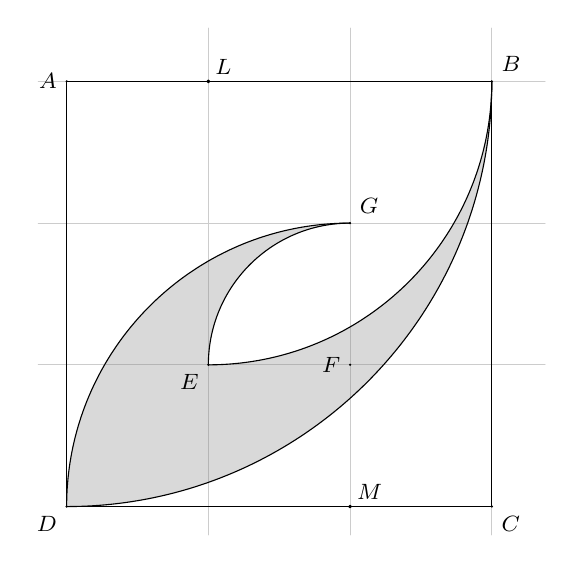
\begin{tikzpicture}[scale=0.45,font=\footnotesize,line join=round,line cap=round,>=stealth]
				\foreach \i in {4,8,12} {
					\draw[color=gray!40, thin] (\i,-0.8) -- (\i,13.5);
					\draw[color=gray!40, thin] (-0.8,\i) -- (13.5,\i);
				}
				
				\draw (0,0) -- (0,12) -- (12,12) -- (12,0) --cycle;
				
				\fill[gray, opacity=0.3] (0,0) arc (-90:0:12) arc (0:-90:8) arc (180:90:4) arc (90:180:8) --cycle;
				
				\draw (0,0) arc (-90:0:12);
				\draw (0,0) arc (180:90:8);
				\draw (4,4) arc (-90:0:8);
				\draw (4,4) arc (180:90:4);
				
				\fill (0,0) circle (1pt) node[below left] {$D$};
				\fill (0,12) circle (1pt) node[left] {$A$};
				\fill (12,12) circle (1pt) node[above right] {$B$};
				\fill (12,0) circle (1pt) node[below right] {$C$};
				\fill (4,4) circle (1pt) node[below left] {$E$};
				\fill (8,4) circle (1pt) node[left] {$F$};
				\fill (8,8) circle (1pt) node[above right] {$G$};
				
				\filldraw (4,12) circle (1pt) node[above right=-1pt] {$L$};
				\filldraw (8,0) circle (1pt) node[above right=-1pt] {$M$};
			\end{tikzpicture}
	\end{center}
	\shortans{37}
	\loigiai{
		\begin{center}
			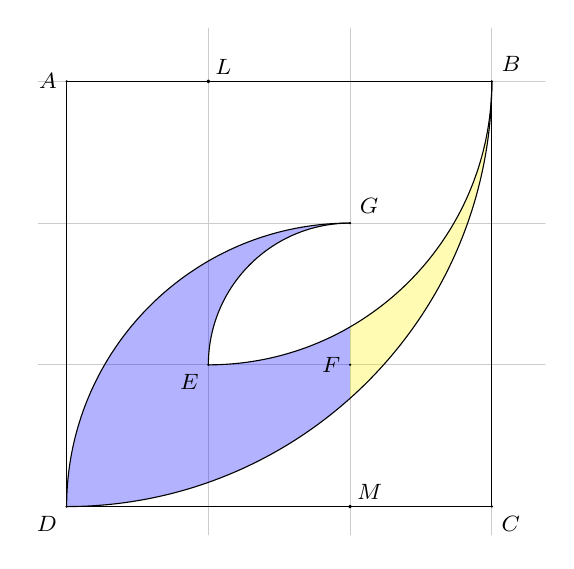
\begin{tikzpicture}[scale=0.45,font=\footnotesize,line join=round,line cap=round,>=stealth]
				\foreach \i in {4,8,12} {
					\draw[color=gray!40, thin] (\i,-0.8) -- (\i,13.5);
					\draw[color=gray!40, thin] (-0.8,\i) -- (13.5,\i);
				}
				
				\def\fullclawpath{(0,0) arc (-90:0:12) -- (12,12) arc (0:-90:8) -- (4,4) arc (180:90:4) -- (8,8) arc (90:180:8) -- cycle;}
				
				\begin{scope}
					\clip (0,-0.8) rectangle (8,13.5);
					\fill[fill=blue, opacity=0.3] \fullclawpath;
				\end{scope}
				
				\begin{scope}
					\clip (8,-0.8) rectangle (12,13.5);
					\fill[fill=yellow, opacity=0.3] \fullclawpath;
				\end{scope}
				
				\draw (0,0) -- (0,12) -- (12,12) -- (12,0) --cycle;
				
				\draw (0,0) arc (-90:0:12);
				
				\draw (0,0) arc (180:90:8);
				
				\draw (4,4) arc (-90:0:8);
				
				\draw (4,4) arc (180:90:4);
				
				\fill (0,0) circle (1pt) node[below left] {$D$};
				\fill (0,12) circle (1pt) node[left] {$A$};
				\fill (12,12) circle (1pt) node[above right] {$B$};
				\fill (12,0) circle (1pt) node[below right] {$C$};
				\fill (4,4) circle (1pt) node[below left] {$E$};
				\fill (8,4) circle (1pt) node[left] {$F$};
				\fill (8,8) circle (1pt) node[above right] {$G$};
				
				\filldraw (4,12) circle (1pt) node[above right=-1pt] {$L$};
				\filldraw (8,0) circle (1pt) node[above right=-1pt] {$M$};
			\end{tikzpicture}
		\end{center}
		Gắn hình trên vào hệ trục toạ độ $Oxy$ như hình vẽ trên.\\
		Ta có $D(0;0)$, $C(12;0)$, $A(0;12)$, $B(12;12)$, $E(4;4)$, $F(8;4)$, $G(8;8)$, $L(4;12)$, $M(8;0)$.\\
		Cung $BD$ là một phần của đường tròn tâm $A$ bán kính $12$ cm.\\
		Ta có $x^2+(y-12)^2=144 \Rightarrow BD \colon y=12-\sqrt{144-x^2}$, $0 \le x \le 12$.\\
		Cung $DG$ là một phần của đường tròn tâm $M$ bán kính $8$ cm.\\
		$(x-8)^2+y^2=64 \Rightarrow DG \colon y=\sqrt{64-(x-8)^2}$, $0 \le x \le 8$.\\
		Cung $EB$ là một phần của đường tròn tâm $L$ bán kính $8$ cm.\\
		$(x-4)^2+(y-12)^2=64 \Rightarrow EB \colon y=12-\sqrt{64-(x-4)^2}$, $4 \le x \le 12$.\\
		Cung $EG$ là một phần của đường tròn tâm $F$ bán kính $4$ cm.\\
		$(x-8)^2+(y-4)^2=16 \Rightarrow EG \colon y=4+\sqrt{16-(x-8)^2}$, $4 \le x \le 8$.\\
		Chia diện tích càng cua thành hai phần, phần một với $0 \le x \le 8$ và phần hai với $8 \le x \le 12$.\\
		Diện tích phần một là
		$$S_1 = \displaystyle\int\limits_0^8 \left| \sqrt{64-(x-8)^2} - \left(12-\sqrt{144-x^2}\right) \right| \mathrm{\,d}x - \displaystyle\int\limits_4^8 \left| \sqrt{16-(x-8)^2} + \sqrt{64-(x-4)^2} - 8 \right| \mathrm{\,d}x \approx 31{,}405$$
		Diện tích phần hai là
		$$S_2 = \displaystyle\int\limits_8^{12} \left| -\sqrt{64-(x-4)^2} + \sqrt{144-x^2} \right| \mathrm{\,d}x \approx 5{,}126$$
		Suy ra, diện tích của càng cua bằng $S = S_1+S_2 \approx 36{,}531 \Rightarrow S \approx 37$ cm$^2$.\\
		Cách 2: Áp dụng công thức tính diện tích hình viên phân có góc ở tâm bằng $90^\circ$ ta có
		$$S = \left(\dfrac{1}{4}\pi R^2 - \dfrac{1}{2}R^2\right) - \left(\dfrac{1}{4}\pi r^2 - \dfrac{1}{2}r^2\right) = \left(\dfrac{1}{4}\pi \cdot 12^2 - \dfrac{1}{2} \cdot 12^2\right) - \left(\dfrac{1}{4}\pi \cdot 4^2 - \dfrac{1}{2} \cdot 4^2\right) \approx 37 \text{ cm$^2$}.$$
	}
\end{ex}

\begin{ex}%[1D9H2-4]
	Dịp cuối tuần một nhóm $27$ bạn gồm Tâm, Vy, Tuệ và $24$ bạn khác cùng nhau đến rạp chiếu phim xem bộ phim \lq\lq Mưa đỏ\rq\rq. Khi xếp tuỳ ý nhóm bạn này vào dãy ghế được đánh số từ $1$ đến $27$, mỗi bạn ngồi một ghế thì xác suất để ghế của Tâm, Vy, Tuệ theo thứ tự lập thành cấp số cộng là $\dfrac{P}{675}$. Tính $P$.
	\shortans{6,5}
	\loigiai{
		Gọi số trên ghế ngồi của ba bạn theo thứ tự lần lượt là $a$, $b$, $c$ ($a$, $b$, $c \in \mathbb{N}^*$; $a$, $b$, $c < 28$).\\
		Theo tính chất của cấp số cộng, ta có $a+c=2b \Rightarrow a$ và $c$ có cùng tính chẵn lẻ.\\
		Dễ thấy rằng, với một bộ $(a,c)$ cùng chẵn hoặc cùng lẻ thì chỉ có duy nhất một giá trị $b$ thoả mãn để $a$, $b$, $c$ tạo thành cấp số cộng.
		\begin{enumerate}[TH 1.]
			\item $a$ và $c$ cùng là số lẻ.\\
			$\Rightarrow$ Có $\mathrm{C}_{14}^2$ cách chọn bộ $(a,c)$ với $a<c$.
			\item $a$ và $c$ cùng là số chẵn.\\
			$\Rightarrow$ Có $\mathrm{C}_{13}^2$ cách chọn bộ $(a,c)$ với $a<c$.
		\end{enumerate}
		Suy ra, số lượng cấp số cộng có thể tạo thành là $\mathrm{C}_{14}^2 + \mathrm{C}_{13}^2 = 169$.\\
		Với mỗi cấp số cộng thoả mãn thì $3$ bạn chỉ có một cách xếp chỗ duy nhất và $24$ bạn còn lại thì có $24!$ cách xếp chỗ vào $24$ ghế.\\
		Để xếp chỗ cho $27$ học sinh thì có $27!$ cách.\\
		Xác suất để số trên ghế ngồi của $3$ bạn tạo thành cáp số cộng là
		$$\dfrac{169 \cdot 24!}{27!} = \dfrac{13}{1350} = \dfrac{\mathrm{P}}{675} \Rightarrow \mathrm{P} = \dfrac{13}{2} = 6{,}5.$$
	}
\end{ex}
\Closesolutionfile{ans}

%\newpage
%\indapan{6}{ans}
